\documentclass[a4paper]{article}
% Kodowanie latain 2
%\usepackage[latin2]{inputenc}
\usepackage[T1]{fontenc}
% Można też użyć UTF-8
\usepackage[utf8]{inputenc}

% Język
\usepackage[polish]{babel}
% \usepackage[english]{babel}

% Rózne przydatne paczki:
% - znaczki matematyczne
\usepackage{amsmath, amsfonts}
% - wcięcie na początku pierwszego akapitu
\usepackage{indentfirst}
% - komenda \url 
\usepackage{hyperref}
% - dołączanie obrazków
\usepackage{graphicx}
% - szersza strona
\usepackage[nofoot,hdivide={2cm,*,2cm},vdivide={2cm,*,2cm}]{geometry}
\frenchspacing
% - brak numerów stron
\pagestyle{empty}
\usepackage{listings}


% dane autora
\author{Barbara Zięba, Dominik Gulczyński}
\title{Dokumentacja projektu Scrabble}
\date{\today}

% początek dokumentu
\begin{document}
\maketitle
\section{Wstęp}
Jako projekt wieńczący kurs Programowania obiektowego napisaliśmy
program umożliwiający przeprowadzenie rozgrywki w Scrabble na
komputerze.
Gra została napisana w języku \texttt{Java}.
Grafika gry powstała na bazie standardowych bibliotek okienkowych \texttt{AWT} i \texttt{Swing}.
\section{Instrukcja dla użytkownika}
\subsection{Początek gry}
Po uruchomieniu programu użytkownik proszony jest o podanie imion graczy.
Gracze będą prowadzili rozgrywkę w podanej kolejności zaczynając od podanego jako pierwszy.
Można podać imiona od jednego do czterech graczy, i to własnie tylu graczy rozpocznie rozgrywkę.
\subsection{Ruch gracza}
Gracz musi w swoim ruchu wykonać jedną z następujących akcji:
\begin{enumerate}
\item[] \textbf{Położenie słowa.} 
Aby położyć słowo gracz powinieć kliknąć kratkę planszy, w której będzie się znajdować pierwsza litera układanego słowa. 
Uwaga: Może to być litera już znajdująca się na planszy.
W nowym okienku należy wpisać jakie to będzie słowo (również litery już znajdujące się na planszy)
i zaznaczyć czy ma zostać położone pionowo (\textit{vertical}) czy poziomo (\textit{horizontal}).
Wszystkie tworzone przy ruchu słowa muszą być poprawne, a dokładane litery łączyć się z już ułożonymi.
Jeśli ruch będzie poprawny odpowiednie litery gracza pojawią się na planszy, a on otrzyma nowe.
\item[] \textbf{Wymiana liter}
Gracz może w swoim ruchu wymienić od jednej do 7 (wszystkich) liter, które posiada.
Za taki ruch nie otrzymuje punktów. 
Aby dokonać wymiany należy kliknąć przycisk \textit{Exchange tiles} znajdujący się obok literek na ręku, a następnie wpisać bez spacji litery do wymiany.
\item[] \textbf{Pass}
Po kliknięciu przycisku \textit{Pass} gracz opuszcza swoją kolejkę.
Może wykonać taki ruch, nawet jeśli ma literki do ułożenia.
\end{enumerate}
Po ruchu litery gracza zostają schowane i pojawia się komunikat o ruchu następnego gracza.
Należy przekazać mu komputer i kliknąć \textit{OK}.
\subsection{Koniec gry}
Gra kończy się, gdy wszyscy gracze z rzędu spasują, lub jeden z graczy wykorzysta wszystkie swoje płytki, a woreczek z płytkami będzie pusty.
Zwycięzcą zostaje gracz o najwyższej liczbie punktów.
Gdy gra kończy się, pojawia się okienko \texttt{EndGameDialog}.
\subsection{Cofanie ruchu}
Gracze sami powinni zdecydować, jak chcą korzystać z tej opcji.
Sugerujemy, żeby w razie pomyłki we wpisywaniu użytkownik mógł zgłosić (niezwłocznie), że chce cofnąć ostatni ruch.
Wtedy następny gracz powinieć skorzystać z przycisku \textit{Revert last move} i dać kolejną szansę koledze.
\subsection{Szczegółowe zasady gry}
Program kopiuje zasady gry Scrabble.
Aby poznać reguły liczenia punktów i inne szczegóły gry, można zajrzeć na stronę \url{http://www.scrabble.info.pl/pobierz/zasady.pdf}.
Nasz program korzysta ze słownika wyrazów dopuszczalnych w grach dostępnego na stronie Słownika Języka Polskiego \url{https://sjp.pl/slownik/growy/}.

\section{Analiza obiektowa}

\subsection{Zaimplementowane klasy}

\subsubsection{Logika gry}

\paragraph{Board} Jedna z głownych klas programu. Przechowuje informacje o stanie planszy: położonych literach, specjalnych polach i słowniku, który decyduje, które wyrazy są poprawne. Posiada dwie metody. Pierwsza, \texttt{placeWord} przyjmuje słowo, które chcemy położyć na planszy i jego pozycję. Jeśli jest to poprawny ruch zwraca parę listę płytek użytych przez gracza i liczbę punktów zdobytych za tej ruch. Kolejna, \texttt{value} służy do liczenia punktów zdobytych za ułożenie danego słowa.

\paragraph{Game} Najważniejsza klasa informująca o przebiegu gry. Dziedziczy z klasy \texttt{Board}, a oprócz tego przechowuje listę graczy, listę ruchów (historię) i woreczek dostępnych literek.
\paragraph{Rack} Po angielsku oznacza stojak na literki. Zawiera listę płytek i udostępnia metody, które pozwalają na aktualizację tej listy.
\paragraph{Player} Klasa dziedzicząca po \texttt{Rack} i odpowiadająca za informacje na temat gracza. Zawiera jego imię i bieżącą liczbę punktów.
\paragraph{Bag} Reprezentuje woreczek z płytkami, które zostały do wylosowania. Jej pole to lista płytek, a metody udostępniają operacje do wykonania na tej liście, np. wyjęcie losowej płytki.
\paragraph{Move} Klasa ruchu. Przydatna do pamiętania historii gry i wyświetlania jej przebiegu.
\paragraph{Tile} Reprezentuje płytkę na planszy. Tutaj mamy również statyczne metody \texttt{getValueOf} (mówi ile punktów jest warta dana litera) i \texttt{paintTile} (służy do rysowania płytek).
\paragraph{Bonus} Odpowiada za specjalne pola planszy. Zawiera informacje informacje na temat bonusów powiększających liczbę punktów zdobywanych za ułożenie słowa. Posiada klasę wewnetrzną \texttt{Type} reprezentującą typy bonusów.
\paragraph{Tree}
Drzewo wyrazów dopuszczonych do użytku w grze. Zostaje utworzone za pomocą pliku txt upublicznionego przez stronę www.sjp.pl. Zawiera wewnętrzną klasę \texttt{Node}. 
\paragraph{Main}
Klasa, która uruchamia program.

\newpage
\subsubsection{Klasy rozszerzające Swing}
\paragraph{Główne okno gry}
\paragraph{\texttt{GameWindow}} Główne okno gry, zarządza komunikacją gracz-komputer.

\begin{figure}[!ht]
\centering
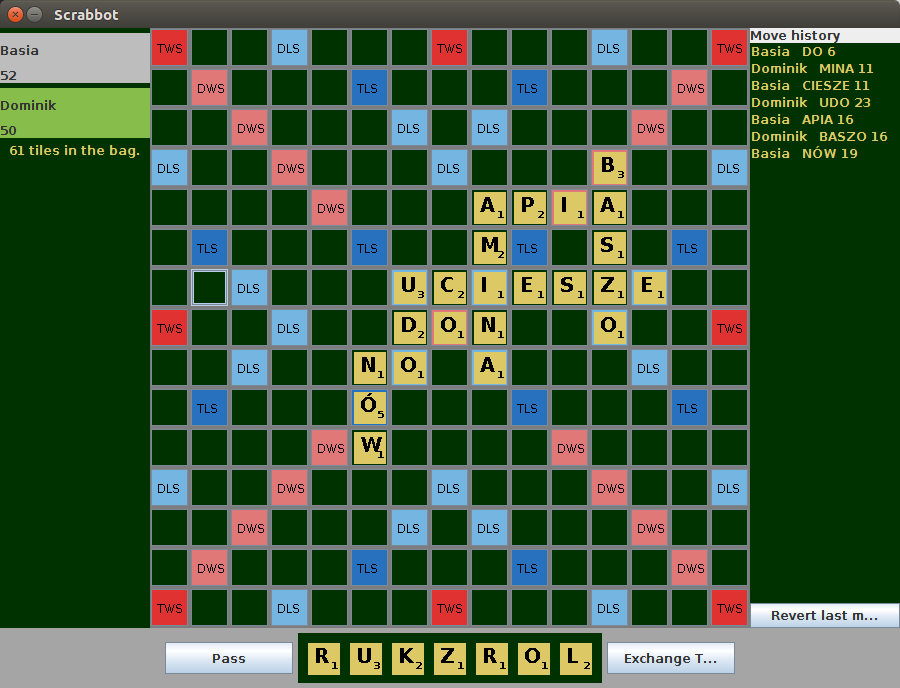
\includegraphics[width=0.7\textwidth]{1.png}
\caption{Główne okno gry}

\end{figure}
\paragraph{Panele}
\paragraph{\texttt{BoardPanel}} Zajmuje centralną część okna gry. Zawiera pola-przyciski typu \texttt{CellButton}, których przyciśnięcie wywołuje \texttt{MoveDialog}.
\paragraph{\texttt{HistoryPanel}} Znajduje się po prawej stronie okna gry. Informuje o historii gry poprzez wypisywanie kolejnych ruchów.
\paragraph{\texttt{PlayerPanel}} Znajduje się po lewej stronie okna gry. Informuje o wynikach poszczególnych graczy. Obecny gracz jest podświetlony na zielono.
\paragraph{\texttt{RackPanel}} Znajduje się na dole okna gry. Wyświetla \texttt{TilePanel} obecnego gracza, oraz zawiera przyciski \texttt{Pass} i \texttt{Exchange}.
\paragraph{\texttt{TilePanel}} Wyświetla stojaczek wybranego gracza.
\paragraph{Przyciski}
\paragraph{\texttt{CellButton}} Wyświetla pojedyncze pole na planszy gry.

\newpage
\paragraph{Okienka typu \textit{pop-up}}
\paragraph{\texttt{EndGameDialog}} Informuje, że gra się zakończyła. Wyświetla tabelę wyników graczy.

\begin{figure}[ht]
\centering
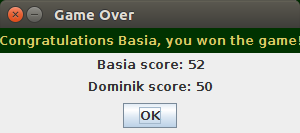
\includegraphics[width=0.3\textwidth]{3.png}
\caption{Okienko zakończenia gry}
\end{figure}

\paragraph{\texttt{ExchangeDialog}} Wyświetla się, gdy gracz, naciśnie przycisk \texttt{Exchange}. Pozwala wymienić literki na stojaczku (kosztuje to jedną turę).
Jeżeli literki które gracz chce wymienić nie zgadzają się z jego stojakiem, pojawia się komunikat o błędzie.

\begin{figure}[!ht]
\centering
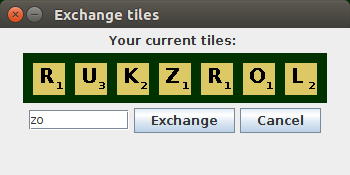
\includegraphics[width=0.3\textwidth]{2.png}
\caption{Okienko wymiany liter}
\end{figure}

\paragraph{\texttt{MoveDialog}} Jest wyświetlany po kliknęciu wybranego pola. W okienku gracz wpisuje wybrane słowo.
Jeśli jest poprawne --- okienko znika, jeśli nie --- pojawia się komunikat o błędzie.

\begin{figure}[!ht]
\centering
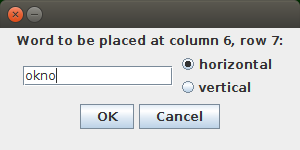
\includegraphics[width=0.3\textwidth]{4.png}
\caption{Okienko nowego ruchu}
\end{figure}

\paragraph{\texttt{NewGameDialog}} Pierwsze okienko, które widzi gracz.
Pozwala wprowadzić do czterech graczy, którzy potem prowadzą rozgrywkę w \texttt{GameWindow}.

\begin{figure}[!ht]
\centering
\includegraphics[width=0.3\textwidth]{5.png}
\caption{Okienko nowej gry}
\end{figure}

\paragraph{\texttt{NewLettersDialog}} Pojawia się zawsze na koniec tury. Informuje gracza o stanie jego stojaczka.

\newpage
\subsection{Diagram UML klas}
Diagramy wygenerowane za pomocą InteliJ IDEA.

\begin{figure}[ht]
\centering
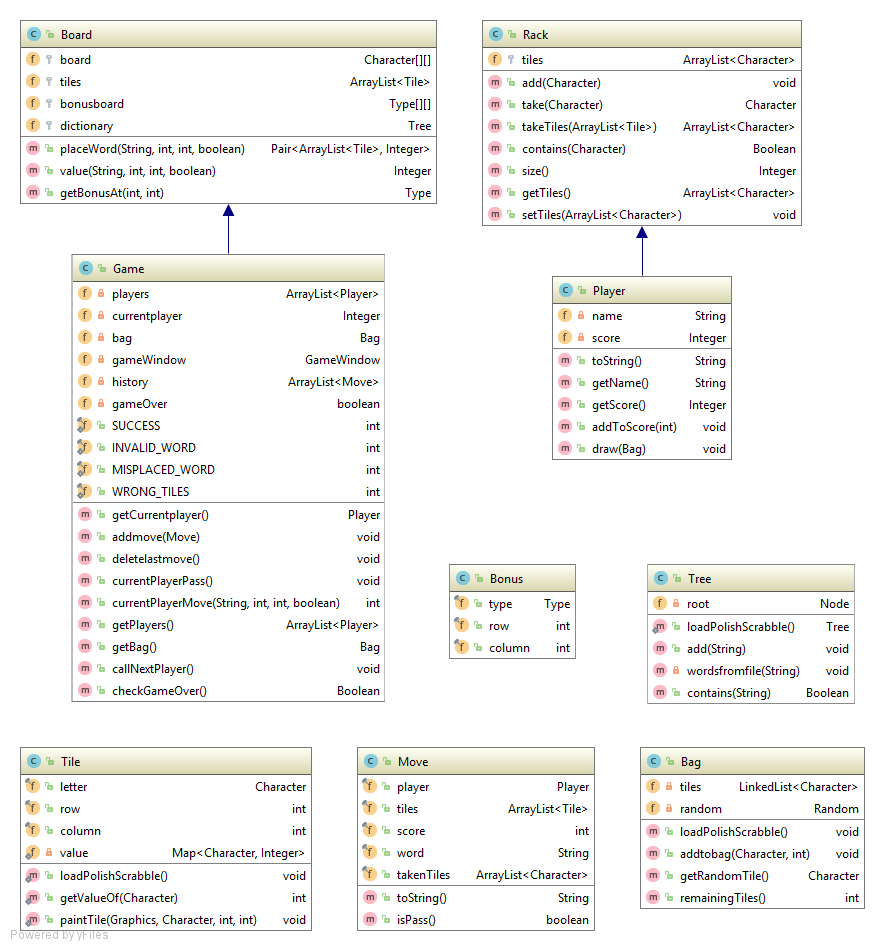
\includegraphics[width=0.5\textwidth]{logika.png}
\caption{Logika gry}
\end{figure}

\begin{figure}[!hb]
\centering
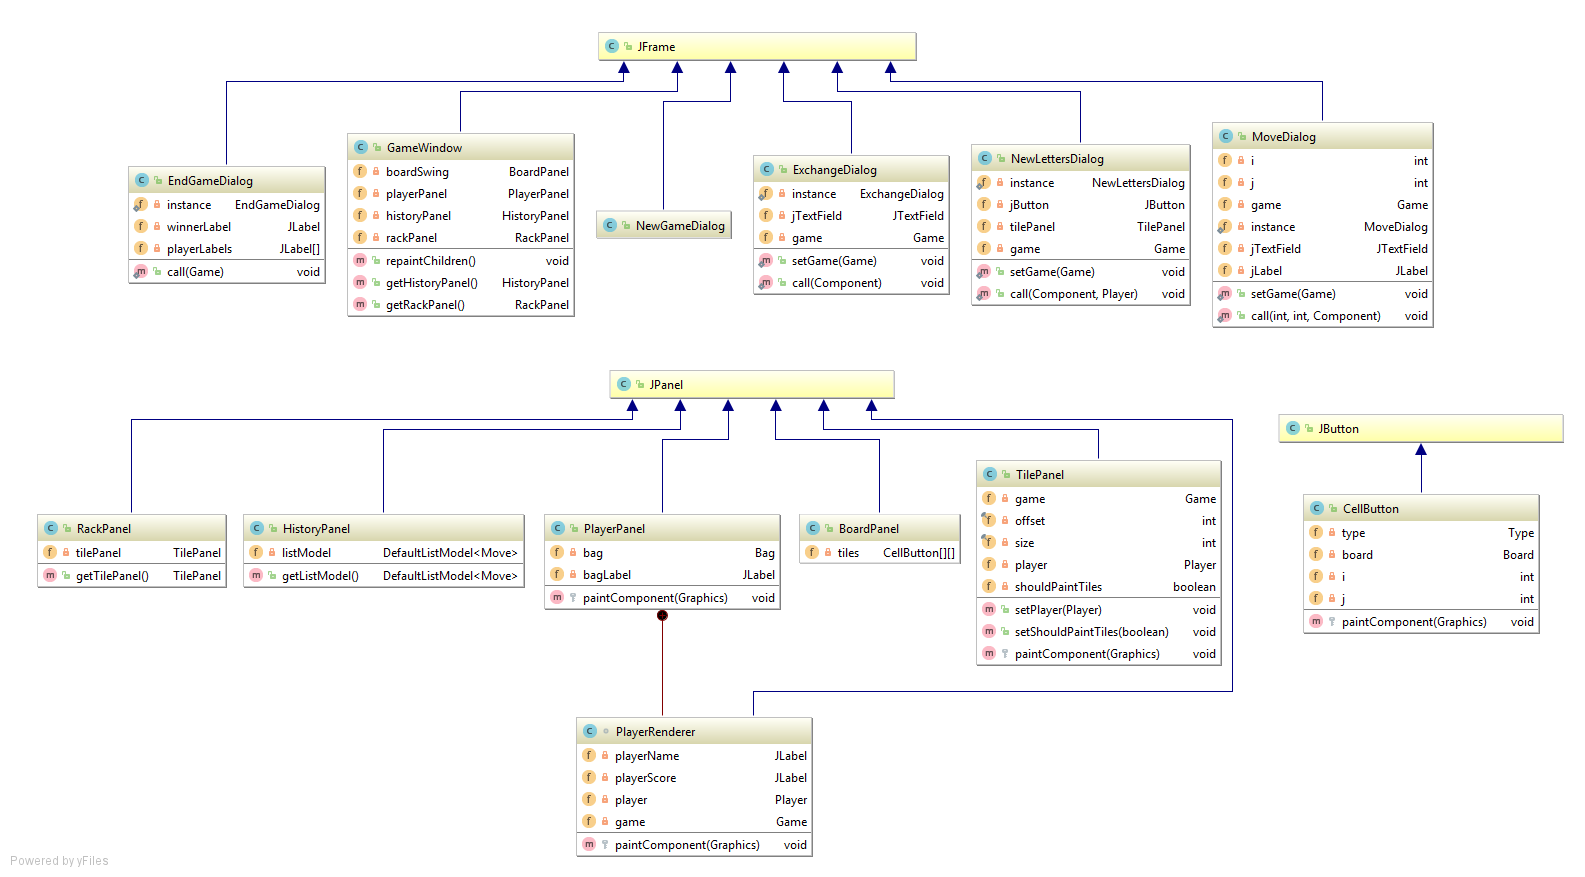
\includegraphics[width=\textwidth]{swing.png}
\caption{Wyświetlanie gry}
\end{figure}

\section{Wskazówki dla programistów}
Projekt jest otwarty na dalszą pracę nad nim. Jedną z opcji jego prostego rozbudowania jest umożliwienie gry w innych językach lub na innych zasadach. Można również pokusić się o dodanie możliwości zmierzenia się w grze z komputerem.
\end{document}